\documentclass{article}\usepackage[]{graphicx}\usepackage[]{color}
% maxwidth is the original width if it is less than linewidth
% otherwise use linewidth (to make sure the graphics do not exceed the margin)
\makeatletter
\def\maxwidth{ %
  \ifdim\Gin@nat@width>\linewidth
    \linewidth
  \else
    \Gin@nat@width
  \fi
}
\makeatother

\definecolor{fgcolor}{rgb}{0.345, 0.345, 0.345}
\newcommand{\hlnum}[1]{\textcolor[rgb]{0.686,0.059,0.569}{#1}}%
\newcommand{\hlstr}[1]{\textcolor[rgb]{0.192,0.494,0.8}{#1}}%
\newcommand{\hlcom}[1]{\textcolor[rgb]{0.678,0.584,0.686}{\textit{#1}}}%
\newcommand{\hlopt}[1]{\textcolor[rgb]{0,0,0}{#1}}%
\newcommand{\hlstd}[1]{\textcolor[rgb]{0.345,0.345,0.345}{#1}}%
\newcommand{\hlkwa}[1]{\textcolor[rgb]{0.161,0.373,0.58}{\textbf{#1}}}%
\newcommand{\hlkwb}[1]{\textcolor[rgb]{0.69,0.353,0.396}{#1}}%
\newcommand{\hlkwc}[1]{\textcolor[rgb]{0.333,0.667,0.333}{#1}}%
\newcommand{\hlkwd}[1]{\textcolor[rgb]{0.737,0.353,0.396}{\textbf{#1}}}%
\let\hlipl\hlkwb

\usepackage{framed}
\makeatletter
\newenvironment{kframe}{%
 \def\at@end@of@kframe{}%
 \ifinner\ifhmode%
  \def\at@end@of@kframe{\end{minipage}}%
  \begin{minipage}{\columnwidth}%
 \fi\fi%
 \def\FrameCommand##1{\hskip\@totalleftmargin \hskip-\fboxsep
 \colorbox{shadecolor}{##1}\hskip-\fboxsep
     % There is no \\@totalrightmargin, so:
     \hskip-\linewidth \hskip-\@totalleftmargin \hskip\columnwidth}%
 \MakeFramed {\advance\hsize-\width
   \@totalleftmargin\z@ \linewidth\hsize
   \@setminipage}}%
 {\par\unskip\endMakeFramed%
 \at@end@of@kframe}
\makeatother

\definecolor{shadecolor}{rgb}{.97, .97, .97}
\definecolor{messagecolor}{rgb}{0, 0, 0}
\definecolor{warningcolor}{rgb}{1, 0, 1}
\definecolor{errorcolor}{rgb}{1, 0, 0}
\newenvironment{knitrout}{}{} % an empty environment to be redefined in TeX

\usepackage{alltt}
\usepackage[margin=1.5cm]{geometry}
\usepackage{microtype} % Slightly better kerning
\usepackage{fixltx2e} % Allow text subscript
\usepackage{graphicx}
\graphicspath{ {./figs/} }
\usepackage[colorlinks=true]{hyperref}
\setlength{\parindent}{0pt}
\setlength{\parskip}{1em}
\usepackage{fancyhdr} % Needed to adjust page numbering
\usepackage{lastpage} % Counts total number of pages

\pagestyle{fancy}
\fancyhf{}
\renewcommand{\headrulewidth}{0pt} % Remove header line
\cfoot{\thepage \hspace{1pt} of \pageref*{LastPage}} % Customize page nums


\usepackage{amsmath}
\usepackage{upgreek}

\title{Forecasting Notes}
\IfFileExists{upquote.sty}{\usepackage{upquote}}{}
\begin{document}
\maketitle

\section{DataCamp: forecasting in R course}

\subsection{Exploring time series}

\begin{itemize}
	\item We can explore time series using the \textit{forecast} package.
	\item We can use the \textit{stats::window()} function to select a segment of a timeseries based on \textit{c(year, period)} (quarter) vs indices
	\item 3 key patters in timeseries
	\begin{itemize}
        \item Trend - long term increase or decrease
        \item Seasonality - regular pattern over fixed period e.g. annual
        \item Cyclical - regular pattern but with no fixed period
    \end{itemize}
    \item \textit{forecast::ggseasonplot()} creates plots by year, rather than continuous
    \item \textit{forecast::ggsubseriesplot()} creates plots by quarter over all years
    \item Lag plots can be used to plot one observation against another (state-space) for autocorrelation
    \begin{itemize}
        \item \textit{forecast::gglagplot()} creates the lag plot
        \item \textit{forecast::ggAcf()} calculates the autocorrelation and creates a plot for each lag
        \item Trends induce positive correlations in the early lags
        \item Seasonality will induce peaks at the seasonal lags
        \item Cyclicity induces peaks at the average cycle length
    \end{itemize}
    \item ``White noise" a purely random time series and is basis of forecasting models
    \begin{itemize}
        \item Can use sampling data of ACF to estimate bounds of significance
        \item Use Ljung-Box test to test a group of autocorrelations together, rather than each separately
        \begin{itemize}
            \item Apply to \textit{diff()} of timeseries
            \item $p < 0.05$ would constitute a ``fail'' as it means there is information in the residuals that hasn't been captured by the model
        \end{itemize}
    \end{itemize}
\end{itemize}

\subsection{Benchmark methods and forecast accuracy}

\begin{itemize}
    \item Run lots of simulations based on statistical model and the mean/median is the ``point forecast"
    \begin{itemize}
        \item Should provide prediction intervals
    \end{itemize}
    \item \textbf{Naive} forecast model is very simple, and provides a baseline for more complicated models, that sometimes don't perform better
    \begin{itemize}
        \item Uses most recent obs as next obs
        \item \textit{forecast::naive()} fits Naive forecast
        \item \textit{forecast::snaive()} fits seasonal Naive forecast
    \end{itemize}
    \item See how good forecast is by testing on data already seen
    \begin{itemize}
        \item Fitted values are forecasts based on all prior values (one-step forecasts)
        \begin{itemize}
            \item When parameters estimated, not really forecasts as all data was used to estimate parameters
        \end{itemize}
        \item Use residuals to evaluate model (\textbf{always check residuals before moving forward with model})
        \begin{itemize}
            \item Residuals should look like (gaussian) white noise if good model
            \item Make 4 assumptions (first two critical, last two convenient)
            \begin{enumerate}
                \item Residuals should be uncorrelated
                    \begin{itemize}
                        \item Otherwise there is information in residuals that should have been captured by forecasting methods
                    \end{itemize}
                \item Residuals have mean zero
                \item Residuals have constant variance
                \item Residuals are normally distributed (required for gaussian white noise vs white noise)
            \end{enumerate}
            \item \textit{forecast::checkresiduals()} plots residuals, autocorrelation, histogram, and performs Ljung-Box test
        \end{itemize}
    \end{itemize}
    \item Forecast errors $\neq$ residuals
    \begin{itemize}
        \item Forecast errors are 
        \begin{itemize}
            \item Errors on \textbf{test} set
            \item Based on multi-step forecasts
        \end{itemize} 
        \item Residuals are 
        \begin{itemize}
            \item Errors on \textbf{training} set
            \item Based on one-step forecasts
        \end{itemize}
    \end{itemize}
    \item Best to use \textbf{Mean Absolute Scaled Error} over \textbf{MAE} or \textbf{MSE} when comparing errors in forecasts on different time series as may have different scales
    \begin{itemize}
        \item $MASE = \frac{MAE}{Q} \text{, where } Q = \text{scaling factor}$
    \end{itemize}
    \item \textit{forecast::accuracy()} computes common metrics used for evaluating both residuals and forecast errors
    \item Cross-validation can be performed in a number of ways
    \begin{itemize}
        \item Multiple one-step forecasts can be made progressively moving forward by one observation each time (rolling origin) and averaging metrics
        \begin{itemize}
            \item Can be applied to multi-step forecasting e.g. two-steps ahead, and three-steps ahead etc
        \end{itemize}
        \item \textit{forecast::tsCV()} can perform cross-validation
        \begin{itemize}
            \item Need to compute own error measures
\begin{knitrout}
\definecolor{shadecolor}{rgb}{0.969, 0.969, 0.969}\color{fgcolor}\begin{kframe}
\begin{alltt}
\hlkwd{library}\hlstd{(forecast)}
\hlkwd{library}\hlstd{(fpp2)}
\hlkwd{library}\hlstd{(tidyverse)}
\hlstd{sq} \hlkwb{<-} \hlkwa{function}\hlstd{(}\hlkwc{u}\hlstd{)\{u}\hlopt{^}\hlnum{2}\hlstd{\}}
\hlkwa{for}\hlstd{(h} \hlkwa{in} \hlnum{1}\hlopt{:}\hlnum{10}\hlstd{)\{}
    \hlstd{oil} \hlopt \hlkwd{tsCV}\hlstd{(}\hlkwc{forecastfunction} \hlstd{= naive,} \hlkwc{h} \hlstd{= h)} \hlopt
    \hlkwd{sq}\hlstd{()} \hlopt \hlkwd{mean}\hlstd{(}\hlkwc{na.rm} \hlstd{=} \hlnum{TRUE}\hlstd{)} \hlopt \hlkwd{print}\hlstd{()}
\hlstd{\}}
\end{alltt}
\begin{verbatim}
## [1] 2355.753
## [1] 4027.511
## [1] 5924.514
## [1] 7950.841
## [1] 9980.589
## [1] 12072.91
## [1] 14054.23
## [1] 15978.92
## [1] 17687.33
## [1] 19058.95
\end{verbatim}
\end{kframe}
\end{knitrout}
        \item Can see how the RMSE is increasing with increasing forecast horizon ($h$)
        \end{itemize}
    \end{itemize}
\end{itemize}

\subsection{Exponential smoothing}

\subsubsection{Simplet exponential smoothing models}
\begin{itemize}
    \item Balance naive and mean forecast models by including all information, but more heavily weighting more recent observations
    \item $\hat{y}_{t+h|t} = \alpha y_t + \alpha(1-\alpha) y_{t-1} + \alpha(1-\alpha)^2 y_{t-2} + \ldots \text{, where } 0 \le \alpha \le 1$
    \begin{itemize}
        \item Describing a function where weights ($\alpha$ terms) decrease exponentially as you go back in time
    \end{itemize}
    \item Equation can be re-written as:
        \begin{itemize}
            \item $\hat{y}_{t+h|t} = \ell_t \text{, where } \ell_t = \alpha y_t + (1 - \alpha)\ell_{t-1}$
            \item $\ell_t$ is known as the ``level" and is the ``smoothing function"
            \begin{itemize}
                \item It is the smoothed value, so updates over time
                \item Need to estimate $\ell_0$, the initial value, and then just update
            \end{itemize}
        \end{itemize}
    \item We choose $\alpha$ and $\ell_0$ to minimize SSE (least squares)
    \begin{itemize}
        \item $SSE = \sum_{t=1}^T \left(y_t - \hat{y}_{t|t-1}\right)^2$
        \begin{itemize}
            \item Have to use this non-linear optimization routine to minimize
        \end{itemize}
    \end{itemize}
    \item \textit{forecast::ses()} function performs simple exponential smoothing
    \item \textit{ggplot2::autolayer(fitted(*ses model*))} useful way of overlaying fitted values as a layer to an \textit{autoplot()} rather than creating a new plot
    \item Only works well when no trend or seasonality
\end{itemize}

\subsubsection{Holt's linear trend model}

\begin{itemize}
    \item Adjusts SES by adding linear trend
    \item Forecast $\hat{y}_{t+h|t} = \ell_t + hb_t$ where:
    \begin{itemize}
        \item $\ell_t = \alpha y_t + (1 - \alpha)(\ell_{t-1} + b_{t-1})$ (``level'')
        \item $b_t = \beta^*(\ell_t - \ell_{t-1}) + (1 - \beta^*)b_{t-1}$ (``trend'')
        \begin{itemize}
            \item $\beta^*$ controls how quickly the slope can change
            \item Because slope can change, often referred to as local linear trend
        \end{itemize}
        \item $0 \le \alpha, \beta^* \le 1$ 
        \item We choose smoothing parameters $\alpha$ and $\beta^*$, and state parameters $\ell_0$ and $b_0$ to minimize SSE (least squares)
    \end{itemize}
    \item A modification can be made to allow the model to ``dampen'' and taper off to a value
    \begin{itemize}
        \item $\hat{y}_{t+h|t} = \ell_t + (\phi + \phi^2 + \ldots + \phi^h)b_t$ (``forecast'')
        \item $\ell_t = \alpha y_t + (1 - \alpha)(\ell_{t-1} + \phi b_{t-1})$ (``level'')
        \item $b_t = \beta^*(\ell_t - \ell_{t-1}) + (1 - \beta^*)\phi b_{t-1}$ (``trend'')
        \item $0 \le \phi \le 1$
        \begin{itemize}
            \item When $\phi = 1$, produces Holt linear trend
        \end{itemize}
    \end{itemize}
\end{itemize}

\subsubsection{Holt-Winter's model}

\begin{itemize}
    \item Adapted to deal with seasonality
    \item Two versions:
    \begin{enumerate}
        \item Additive
            \begin{itemize}
                \item $\hat{y}_{t+h|t} = \ell_t + hb_t + s_{t-m+h_m^+}$ (``forecast'')
                \item $\ell_t = \alpha (y_t - s_{t-m})+ (1 - \alpha)(\ell_{t-1} + b_{t-1})$ (``level'')
                \item $b_t = \beta^*(\ell_t - \ell_{t-1}) + (1 - \beta^*) b_{t-1}$ (``trend'')
                \item $s_t = \gamma (y_t - \ell_{t-1} - b_{t-1}) + (1-\gamma)s_{t-m}$
                \item $s_{t-m+h_m^+}$ is a seasonal component
                \begin{itemize}
                    \item $m$ is the period of seasonality e.g. quarter
                    \item seasonal component averages \textbf{zero}
                \end{itemize}
                \item $0 \le \alpha \le 1, 0 \le \beta^* \le 1, 0 \le \gamma \le 1-\alpha$
            \end{itemize}
        \item Multiplicative
        \begin{itemize}
            \item $\hat{y}_{t+h|t} = \ell_t + hb_t + s_{t-m+h_m^+}$ (``forecast'')
            \item $\ell_t = \alpha \frac{y_t}{ s_{t-m}} + (1 - \alpha)(\ell_{t-1} + b_{t-1})$ (``level'')
            \item $b_t = \beta^*(\ell_t - \ell_{t-1}) + (1 - \beta^*) b_{t-1}$ (``trend'')
            \begin{itemize}
                \item Trend is stil linear
            \end{itemize}
            \item $s_t = \gamma \frac{y_t}{\ell_{t-1} - b_{t-1}} + (1-\gamma)s_{t-m}$
            \begin{itemize}
                \item Seasonality is now multiplicative
            \end{itemize}
            \item $s_{t-m+h_m^+}$ is a seasonal component
            \begin{itemize}
                \item $m$ is the period of seasonality e.g. quarter
                \item seasonal component averages \textbf{one}
            \end{itemize}
            \item $0 \le \alpha \le 1, 0 \le \beta^* \le 1, 0 \le \gamma \le 1-\alpha$
            \item Use multiplicative when seasonal variation increases with the level of the series (as time goes on the smoothed value increases)
        \end{itemize}
    \end{enumerate}
    \item Can add damping to trend of HW models, as with Holt's linear trend models
    \begin{itemize}
        \item Damping can be either additive or multiplicative, however, multiplicative trend damping generally doesn't work well
    \end{itemize}
    \item \textit{forecast::hw()} is used for the Holt-Winter's (and therefore Holt's linear trend) models\
    \begin{itemize}
        \item Set \textit{seasonality = ``additive/multiplicative''}
    \end{itemize}
\end{itemize}

\subsubsection{ Innovations state space models}

\begin{itemize}
    \item The exponential smoothing models discussed are known as \textbf{state space} models
    \begin{itemize}
        \item Each model consists of an equation that describes the observed data, and some state equations that describe how the unobserved components or states (level, trend, seasonal) change over time
        \item To demonstrate, let's look at an SES model
        \begin{enumerate}
            \item Recall $\hat{y}_{t+h|t} = \ell_t$ and $\ell_t = \alpha y_t + (1-\alpha)\ell_{t-1}$
            \item Rewrite the level function in the ``error correction'' form
            \begin{itemize}
                \item $\ell_t = \alpha y_t + (1-\alpha)\ell_{t-1}$
                \item $\ell_t = \ell_{t-1} + \alpha(y_t - \ell_{t-1})$
                \item $\ell_t = \ell_{t-1} + \alpha e_t$ where:
                \begin{itemize}
                    \item $e_t = y_t - \ell_{t-1}$
                    \item $e_t = y_t - \hat{y}_{t|t-1}$
                    \item $e_t$ is therefore the residual at time $t$
                \end{itemize}
                \item Assuming residuals are normally and independently distributed with mean 0 and variance $\sigma^2$ ($e_t = \upvarepsilon_t \sim NID(0, \sigma^2))$
            \end{itemize}
            \item Rewrite \textit{measurement} and \textit{state} equations
            \begin{itemize}
                \item $y_t = \ell_{t-1} - \upvarepsilon_t$
                \item $\ell_t = \ell_{t-1} + \alpha \upvarepsilon_t$
            \end{itemize}
        \end{enumerate}
    \end{itemize}
    \item Additive and multiplicative models will produce the same ``point forecast'', however, they will differ in their prediction intervals as they will exhibit different errors
    \item We can label state space models as \textbf{ETS} models (Error, Trend, Seasonal) with the following possible labels:
    \begin{itemize}
        \item Error = $\{A, M\}\text{, where } A,M = \text{Additive, Multiplicative}$
        \item Trend = $\{N, A, A_d\} \text{, where } N, A_d = \text{None, Additive damped}$
        \item Seasonal = $\{N, A, M\}$
    \end{itemize}
    \item Multiplicative errors means noise increases with the level of the series (prediction intervals get much wider than additive)
    \item ETS is useful as it allows us to:
    \begin{itemize}
        \item Use MLE to optimize parameters
        \item Generate prediction intervals for all models
        \item Automatically select the best exponential smoothing model for timeseries
        \begin{itemize}
            \item Minimize bias-corrected version of AIC (AIC\textsubscript{c})
            \begin{itemize}
                \item Similar to cross-validation, but much faster
                \item Equivalent to minimizing SSE in models with additive errors
            \end{itemize}
        \end{itemize}
    \end{itemize}
    \item \textit{forecasts::ets()} automatically selects ETS model using AIC\textsubscript{c}
    \begin{itemize}
        \item Need to pass to \textit{forecast::forecast()} function for predictions
    \end{itemize}
    \item ETS models are not necessarily better than simpler ones e.g. seasonal naive
\end{itemize}

\subsection{Forecasting with ARIMA models}

\begin{itemize}
        \item ETS use multiplicative errors and seasonality to handle variance that increases with levels
    \begin{itemize}
        \item Can use transformations to adjust instead
    \end{itemize}
    \item Box-Cox transformations used to create common variance
    
    \[ 
        w_t = \begin{cases}
        \log(y_t) & \lambda = 0 \\
        \left(y_t^\lambda - 1\right)/\lambda & \lambda \neq 0
        \end{cases}
    \]

    \begin{itemize}
        \item \textit{forecast::BoxCox.lambda()} will select best value of $\lambda$
        \item Essential to use transformation of some kind with ARIMA models
    \end{itemize}
    \item Non-seasonal autoregressive integrated moving average models
    \begin{itemize}
        \item Autoregressive models are regression of time series against lagged \textbf{values} of series
        \item Moving average models are regression against lagged \textbf{errors}
        \item Adding two you get an ARMA model
        \begin{itemize}
            \item Last $p$ observations, and last $q$ errors are used as predictors in the equation
            \item Can only work with stationary data so need to difference data first
            \begin{itemize}
                \item Stationary timeseries have properties that don't depend on the time i.e. no trends or seasonal components, but can have cyclical patterns
            \end{itemize}
        \end{itemize}
        \item \textbf{Integrated} is the opposite of differencing (e.g. integration vs differentiation)
        \begin{itemize}
            \item If timeseries needs to be differenced $d$ times, known as ARIMA ($p, d, q$) model
            \begin{itemize}
                \item d = number of lag-1 differences
                \item p = number of ordinary AR lags: $y_{t-1}, y_{t-2}, \ldots, y_{t-p}$
                \item q = number of ordinary MA lags: $\varepsilon_{t-1}, \varepsilon_{t-2}, \ldots, \varepsilon_{t-q}$
            \end{itemize}
        \end{itemize}
        \item \textit{forecast::auto.arima()} automatically selects best values of $p, d, q$ by minimizing AIC\textsubscript{c}
        \begin{itemize}
            \item Parameters estimated using MLE
            \item Can only compare AIC\textsubscript{c} values between models of same class (e.g. ARIMA vs ARIMA, not ARIMA vs ETS) and same differencing
            \item Stepwise search to test parameters means that may find local minimum
            \item \textit{drift} term refers to $c$, which is the average change between consecutive observations 
        \end{itemize}
        \item Use cross-validation to compare models of different classes
        \begin{itemize}
            \item Find MSE of each class
            
\begin{knitrout}
\definecolor{shadecolor}{rgb}{0.969, 0.969, 0.969}\color{fgcolor}\begin{kframe}
\begin{alltt}
\hlkwd{library}\hlstd{(tidyverse)}
\hlkwd{library}\hlstd{(forecast)}
\hlkwd{library}\hlstd{(fpp2)}

\hlcom{# ETS function for CV}
\hlstd{fets} \hlkwb{<-} \hlkwa{function}\hlstd{(}\hlkwc{x}\hlstd{,} \hlkwc{h}\hlstd{) \{}
    \hlkwd{forecast}\hlstd{(}\hlkwd{ets}\hlstd{(x),} \hlkwc{h} \hlstd{= h)}
\hlstd{\}}
\hlcom{# ARIMA function for CV}
\hlstd{farima} \hlkwb{<-} \hlkwa{function}\hlstd{(}\hlkwc{x}\hlstd{,} \hlkwc{h}\hlstd{) \{}
    \hlkwd{forecast}\hlstd{(}\hlkwd{auto.arima}\hlstd{(x),} \hlkwc{h}\hlstd{=h)}
\hlstd{\}}

\hlcom{# Compute CV errors for ETS on austa as e1}
\hlstd{e1} \hlkwb{<-} \hlkwd{tsCV}\hlstd{(austa, fets,} \hlkwc{h} \hlstd{=} \hlnum{1}\hlstd{)}

\hlcom{# Compute CV errors for ARIMA on austa as e2}
\hlstd{e2} \hlkwb{<-} \hlkwd{tsCV}\hlstd{(austa, farima,} \hlkwc{h} \hlstd{=} \hlnum{1}\hlstd{)}

\hlcom{# Find MSE of each model class}
\hlkwd{mean}\hlstd{(e1}\hlopt{^}\hlnum{2}\hlstd{,} \hlkwc{na.rm} \hlstd{=} \hlnum{TRUE}\hlstd{)}
\end{alltt}
\begin{verbatim}
## [1] 0.05623684
\end{verbatim}
\begin{alltt}
\hlkwd{mean}\hlstd{(e2}\hlopt{^}\hlnum{2}\hlstd{,} \hlkwc{na.rm} \hlstd{=} \hlnum{TRUE}\hlstd{)}
\end{alltt}
\begin{verbatim}
## [1] 0.04336277
\end{verbatim}
\end{kframe}
\end{knitrout}

        \end{itemize}
    \end{itemize}
    \item Seasonal ARIMA
    \begin{itemize}
        \item Uses same parameters, but uppercase to signify seasonal
        \begin{itemize}
            \item D = number of seasonal differences
            \item P = number of seasonal AR lags: $y_{t-m}, y_{t-2m}, \ldots, y_{t-Pm}$
            \item Q = number of seasonal MA lags: $\varepsilon_{t-m}, \varepsilon_{t-m}, \ldots, \varepsilon_{t-Qm}$
            \item m = seasonal period (number of observations per year)
        \end{itemize}
        \item Non-linear as seasonal components multiply with non-seasonal components
        \item Allow seasonality to \textbf{change over time}
        \begin{itemize}
            \item Mainly affected by seasonality at end of series, and not as much by the start
        \end{itemize}
        \item When using \textbf{at least two differences}, forecast will have trend without needing to include drift term (e.g. ordinary and seasonal differencing)
    \end{itemize}
\end{itemize}

\subsection{Advanced methods}

\begin{itemize}
    \item Often want to include information from other variables to improve our forecast (rather than just relying on changes in outcome variable)
    \item Dynamic regression
    \begin{itemize}
        \item $y_t = \beta_0 + \beta_1 x_{1, t} + \ldots + \beta_r x_{r, t} + e_t$
        \begin{itemize}
            \item  Looks very similar to standard linear regression equation, but error term is ARIMA process
        \end{itemize}
        \item \textit{forecast::auto.arima(df[, ``outcome''], xreg = df[, ``var''])} used to fit dynamic regression model
        \item \textit{forecast::forecast(fit, xreg = rep(value, period))} used to forecast different scenarios of the input variable (value and period)
    \end{itemize}
    \item Dynamic harmonic regression
    \begin{itemize}
        \item Uses Fourier terms to account for seasonality
        \item $y_t = \beta_0 + \beta_1 x_{1, t} + \ldots + \beta_{t, r}x_{t, r} + \sum_{k=1}^K \left[\alpha_k s_k(t) + \gamma_k c_k (t)\right] + e_t$
        \begin{itemize}
            \item $s_k(t)=\sin\left(\frac{2kt}{m}\right)$
            \item $c_k(t)=\cos\left(\frac{2kt}{m}\right)$
            \item $m=$ seasonal period
            \item Usually don't use ARIMA errors as seasonality already accounted for
            \item Assume seasonal pattern doesn't change over time
        \end{itemize}
        \item \textit{forecast::auto.arima(df, xreg = fourier(df, K = k), seasonal = FALSE, lambda = w)} fits dynamic harmonic regression
        \begin{itemize}
            \item Select $K$ to minimize AIC\textsubscript{c} (cross-validation?)
            \item $K < \frac{m}{2}$
            \item \textit{seasonal = FALSE} indicates don't want to produce ARIMA errors
        \end{itemize}
        \item \textit{fit \%$>$\% forecast::forecast(xreg = fourier(df, K = k, h = h))} forecasts using the dynamic harmonic regression model
        \begin{itemize}
            \item Selecting \textit{h} indicates want to forecast forward
        \end{itemize}
        \item Fourier terms vs ARIMA is that handles large values of $m$ well 
        \begin{itemize}
            \item E.g. seasonal period of weekly data approx 52
            \item When annual seasonality with daily data ($m=365$)
        \end{itemize}
\begin{knitrout}
\definecolor{shadecolor}{rgb}{0.969, 0.969, 0.969}\color{fgcolor}\begin{kframe}
\begin{alltt}
\hlkwd{library}\hlstd{(tidyverse)}
\hlkwd{library}\hlstd{(forecast)}
\hlkwd{library}\hlstd{(fpp2)}

\hlcom{# Set up harmonic regressors of order 13}
\hlstd{harmonics} \hlkwb{<-} \hlkwd{fourier}\hlstd{(gasoline,} \hlkwc{K} \hlstd{=} \hlnum{13}\hlstd{)}

\hlcom{# Fit regression model with ARIMA errors}
\hlstd{fit} \hlkwb{<-} \hlkwd{auto.arima}\hlstd{(gasoline,} \hlkwc{xreg} \hlstd{= harmonics,} \hlkwc{seasonal} \hlstd{=} \hlnum{FALSE}\hlstd{)}

\hlcom{# Forecasts next 3 years}
\hlstd{newharmonics} \hlkwb{<-} \hlkwd{fourier}\hlstd{(gasoline,} \hlkwc{K} \hlstd{=} \hlnum{13}\hlstd{,} \hlkwc{h} \hlstd{=} \hlnum{52}\hlopt{*}\hlnum{3}\hlstd{)}
\hlstd{fc} \hlkwb{<-} \hlkwd{forecast}\hlstd{(fit,} \hlkwc{xreg} \hlstd{= newharmonics)}

\hlcom{# Plot forecasts fc}
\hlkwd{autoplot}\hlstd{(fc)}
\end{alltt}
\end{kframe}
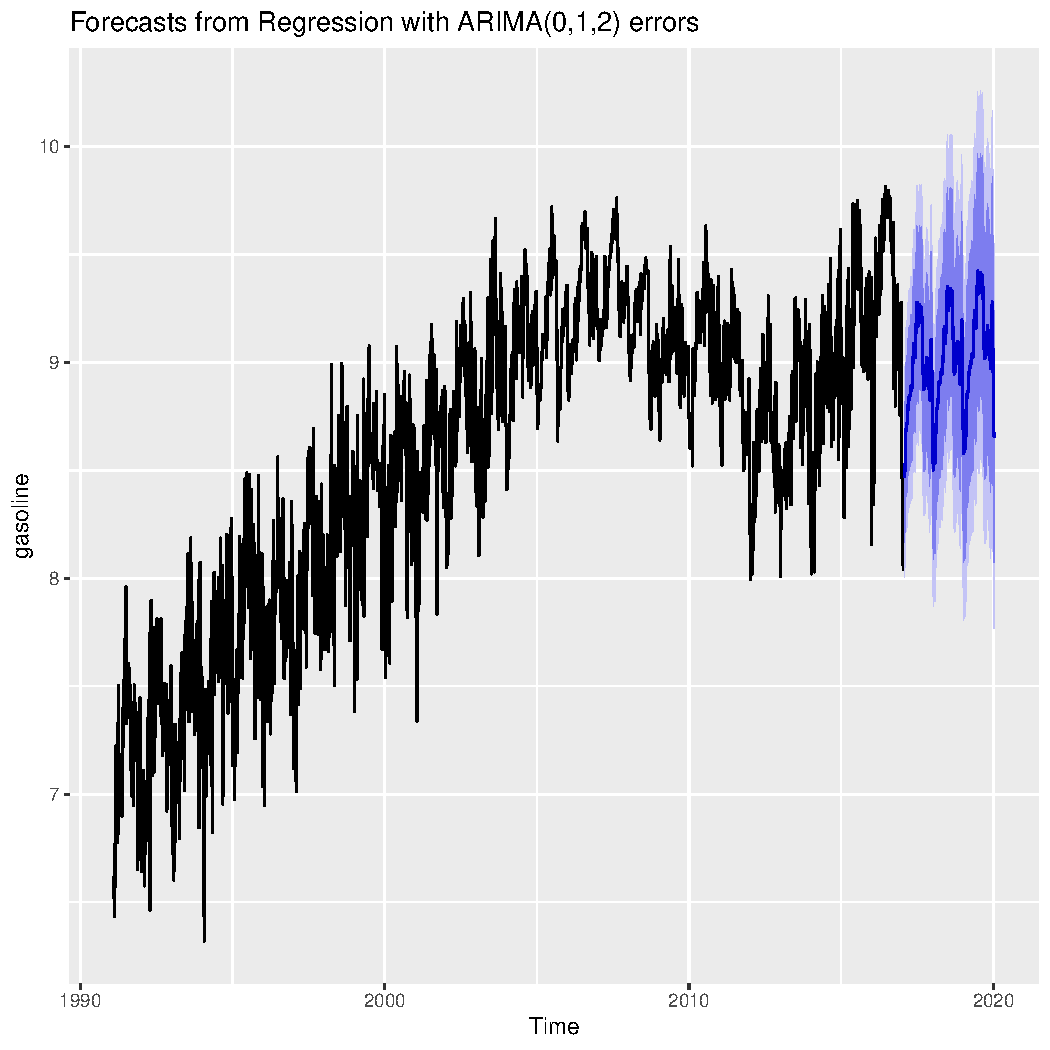
\includegraphics[width=\maxwidth]{figure/unnamed-chunk-3-1} 

\end{knitrout}

        \item Harmonic regressions are useful when there is multiple seasonality in a timeseries e.g. daily and weekly seasonality
        \begin{itemize}
            \item Need to specify both values of $K$ in \textit{fourier()} e.g. \textit{fourier(df, K = c(10, 10))}
            \item \textit{forecast(fit, newdata = data.frame(fourier(df, K = c(10, 10), h = 20*48)))}
        \end{itemize}
        \item Sometimes \textit{forecast::auto.arima()} is too slow when fitting very long timeseries (particularly with multiple seasonality), so use Fourier terms in \textit{forecast::tslm()} function
        \begin{itemize}
            \item \textit{tslm(df $\sim$ fourier(df, K = c(10, 10)))}
            \item Works like regular \textit{lm()}
        \end{itemize}
    \end{itemize}
    \item TBATS model
    \begin{itemize}
        \item \textbf{T}rigonometric terms for seasonality
        \begin{itemize}
            \item Allows seasonality to change over time, unlike Fourier terms
        \end{itemize}
        \item \textbf{B}ox-Cox transformation for homogeneity
        \item \textbf{A}RMA errors for short-term dynamics
        \item \textbf{T}rend and level terms, including damping, like ETS model
        \item \textbf{S}easonal (including multiple and non-integer periods)
        \item Very general and handles large range of timeseries
        \item Very useful for timeseries with large seasonal periods and multiple seasonal periods
        \item Have to be careful with its automation
        \begin{itemize}
            \item Point forecast often good
            \item Prediction intervals can be very wide
            \item Slow with large timeseries
        \end{itemize}
        \item \textit{forecast::tbats(df)} used to fit model
    \end{itemize}
\end{itemize}








\end{document}
